

\documentclass{article}

\usepackage{amsmath}
\usepackage{graphicx}
\graphicspath{ {images/} }
\usepackage{hyperref}
\hypersetup{
    colorlinks=true,
    linkcolor=blue,
    filecolor=magenta,      
    urlcolor=cyan,
}
\usepackage{geometry}
 \geometry{
 a4paper,
 total={170mm,267mm},
 left=20mm,
 top=20mm,
 }

\title {De-Anonymizing Social Network Users}
\author{Dixita Sharegar}
\date{Monday, February 8, 2016}
\begin{document}
\maketitle
Millions of users use social networking sites to share personal and business related information on websites like Facebook, LinkedIn and Xing. Although these websites try to protect the user’s data, there are always new ways to attack and extract sensitive information. The paper “A Practical Attack to De-Anonymize Social Network Users” presents a technique of obtaining the identity of a user from his group membership. If a user visits the attacker’s website, then the attacker can get enough information to uniquely identify the user. If not, then the attacker at least gets a smaller subset of data to work with.Sites like Amazon and eBay also use the concepts of groups and are prone to such attacks. \\
\par Every social network model is a graph of \textit{V} users and \textit{E} edges representing friendship between them. Social networks also have groups \textit{G} where many users with common interests or demographics join. A user can belong to multiple groups where every individual group is represented by \textit{g}. To represent this data we use a vector :

\begin{equation}
T(v):=(T_g(v))_{g \epsilon G}
\end{equation}

$$T_g(v)= 
\left
 \{
  \begin{tabular}{ccc}
  1 if v is a member of a group g\\
  0 if v is not a member of a group g
  \end{tabular}
\right \}$$


 \(T(v)\)  is called the group fingerprint of the user. This information will be used in the deanonymizing attack. \\
\par Web applications use HTTP GET parameters to communicate with the users. These hyperlinks contain user IDs or group IDs that help the attacker to identify a user or group. The first step to de-anonymizing attack is that the attacker sends a list of hyperlinks to the user’s browser. Next, by using client side scripting, he forces the user’s browser to check the list with the user’s browsing history. At the end, the attacker gets a list of visited URLs.

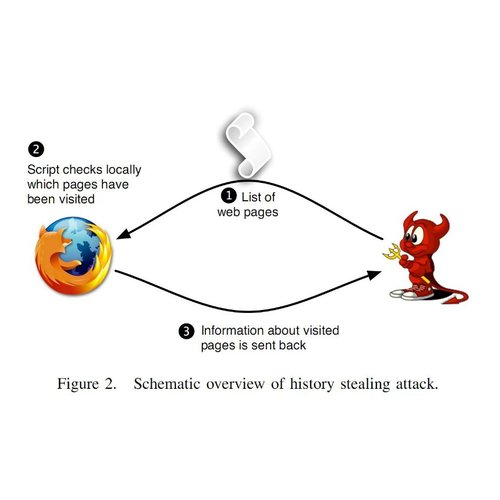
\includegraphics[scale=0.7]{HistoryStealing}

 This paper discusses 2 models, the basic attack and the improved attack.

\begin{enumerate}
\item Basic Attack: The attacker would first study the social network, the dynamic URL pattern, the numbering pattern of IDs etc. and then perform the attack. This attack is not feasible as every potential victim’s browser has to perform a lot of data processing and is time consuming.
\item  Improved Attack: The attacker studies the social network like above. Then he steals the user’s browsing history and checks if group pages were recently accessed. If we find a matching page we assume that the user is a member of that group. We can now generate the candidte set and de-anonymize the user.

\end{enumerate}

Web crawling techniques can also be used to get user data. A custom crawler and a third party crawler were used to test this attack on social networking sites like Facebook, LinkedIn and Xing .Data for 1.8 million unique users was obtained from 6,446 public and 108 private groups in Xing.The problem with this technique is that the data gathered by the attacker can be inconsistent as users could have deleted their browsing history, members are added and deleted to groups, so data needs to be collected by the attacker on a regular basis.\\

We can mitigate the attacks either at the server side or client side. At the server side we should try using HTTP POST instead of GET as GET parameters are stored in browsing history. Users should disable browser history or use private browsing mode. At Xing they have added random numeric characters that represent current date and user number to their URLs to solve the problem.

\begin{thebibliography}{9}

\bibitem{reference}
  Wondracek, G.;Holz, T.;Kirda, E.;Kruegel, C.,
  \emph{A Practical Attack to De-anonymize Social Network Users},
  2010 IEEE Symposium on,vol., no., pp.223-238,
  16-19 May 2010.

\end{thebibliography}

\href{http://goo.gl/mmM16L}{History Stealing Image Link}

\href{https://github.com/dixita90/Security-Algorithms-Protocols.git}{GitHub Repository Link}

\end{document}